\documentclass[11pt, a4paper, titlepage, openright]{article}
% \usepackage[options]{package}

\title{\LARGE Scientific Programming \\ \normalsize Data Fitting Exercise 1}
\author{Armin Halilovic - s0122210}
\date{October 30, 2015}

\usepackage[font=small,labelfont=bf]{caption}
\usepackage{float}
%\floatstyle{boxed}
\restylefloat{figure}
\usepackage{graphicx}
\usepackage{hyperref}
\usepackage{mathtools}
%\usepackage{titlesec}
\usepackage[titletoc, title]{appendix}
\usepackage{listings}
\usepackage{color}

\definecolor{dkgreen}{rgb}{0,0.6,0}
\definecolor{gray}{rgb}{0.5,0.5,0.5}
\definecolor{mauve}{rgb}{0.58,0,0.82}

\lstset{frame=tb,
  language=C++,
  aboveskip=3mm,
  belowskip=3mm,
  showstringspaces=false,
  columns=flexible,
  basicstyle={\footnotesize\ttfamily},
  numbers=none,
  numberstyle=\tiny\color{gray},
  keywordstyle=\color{blue},
  commentstyle=\color{dkgreen},
  stringstyle=\color{mauve},
  breaklines=true,
  breakatwhitespace=true,
  tabsize=3,
  showstringspaces=false
}

\begin{document}
%%%%%%%%%%%%%%%%%%%%%%%%%%%%%%%%%%%%%%%%%
% University Assignment Title Page
% LaTeX Template
% Version 1.0 (27/12/12)
%
% This template has been downloaded from:
% http://www.LaTeXTemplates.com
%
% Original author:
% WikiBooks (http://en.wikibooks.org/wiki/LaTeX/Title_Creation)
%
% License:
% CC BY-NC-SA 3.0 (http://creativecommons.org/licenses/by-nc-sa/3.0/)
%
% Instructions for using this template:
% This title page is capable of being compiled as is. This is not useful for
% including it in another document. To do this, you have two options:
%
% 1) Copy/paste everything between \begin{document} and \end{document}
% starting at \begin{titlepage} and paste this into another LaTeX file where you
% want your title page.
% OR
% 2) Remove everything outside the \begin{titlepage} and \end{titlepage} and
% move this file to the same directory as the LaTeX file you wish to add it to.
% Then add \input{./title_page_1.tex} to your LaTeX file where you want your
% title page.
%
%%%%%%%%%%%%%%%%%%%%%%%%%%%%%%%%%%%%%%%%%

%----------------------------------------------------------------------------------------
%	PACKAGES AND OTHER DOCUMENT CONFIGURATIONS
%----------------------------------------------------------------------------------------
\begin{titlepage}

\newcommand{\HRule}{\rule{\linewidth}{0.5mm}} % Defines a new command for the horizontal lines, change thickness here

\center % Center everything on the page

%----------------------------------------------------------------------------------------
%	HEADING SECTIONS
%----------------------------------------------------------------------------------------

\textsc{\LARGE University of Antwerp}\\[1.5cm] % Name of your university/college
\textsc{\Large }\\[4cm] % Major heading such as course name
\textsc{\Large Scientific Programming}\\[0.5cm] % Minor heading such as course title

%----------------------------------------------------------------------------------------
%	TITLE SECTION
%----------------------------------------------------------------------------------------

\HRule
{ \huge \bfseries Second Session \\ \Large{Exercise 2}}\\ % Title of your document
\HRule \\[1.5cm]

%----------------------------------------------------------------------------------------
%	AUTHOR SECTION
%----------------------------------------------------------------------------------------

\begin{minipage}{0.4\textwidth}
\begin{flushleft} \large
Armin Halilovic - s0122210 % Your name
\end{flushleft}
\end{minipage}
~
\begin{minipage}{0.4\textwidth}
\begin{flushright} \large
\end{flushright}
\end{minipage}\\[4cm]

% If you don't want a supervisor, uncomment the two lines below and remove the section above
%\Large \emph{Author:}\\
%John \textsc{Smith}\\[3cm] % Your name

%----------------------------------------------------------------------------------------
%	DATE SECTION
%----------------------------------------------------------------------------------------

\vfill % Fill the rest of the page with whitespace
{\large August 22, 2016}\\[3cm] % Date, change the \today to a set date if you want to be precise

%----------------------------------------------------------------------------------------
%	LOGO SECTION
%----------------------------------------------------------------------------------------

%\includegraphics{Logo}\\[1cm] % Include a department/university logo - this will require the graphicx package

%----------------------------------------------------------------------------------------


\end{titlepage}
\onecolumn
\tableofcontents
\newpage
%\twocolumn



\section{Problem}
    We are given the Runge function  \[f(x) = \frac{1}{1 + 25 x^{2}} \ \ x \in [-1, 1] \]
    We will construct graphs that approximate this function using a few interpolation techniques. \\
    First, we will use Newton's divided differences interpolation on a set of equidistant and a set of non equidistant points.
    Then, cubic spline interpolation will be used, followed by spline interpolation with modified boundary conditions.

    All of this will be done using C++ and the \href{http://www.gnu.org/software/gsl/}{GNU Scientific Library}.
    In the solutions, we will briefly describe what we did with excerpts from the code, generate graphs using the interpolation methods,
    and look at how close each one of them got to the Runge function. The first solution will contain more information than
    the other ones, as it will explain most of the code.

\section{Using the code}
    All of the C++ code can be found in the "main.cpp" file and in appendix A of this document.
    main.cpp comes accompanied by createImages.sh, which contains all of the neccessary UNIX commands to generate the graph images.
    This file relies on the \href{https://www.gnu.org/software/plotutils/manual/en/html_node/graph.html}{graph} program
    in the GNU plotutils package to plot graphs, so make sure that it is installed.

    To compile and run the program, execute the following commands in the build/ directory:
    \begin{lstlisting}
    cmake ..
    make
    chmod +x ./createImages.sh
    ./data_fitting
    \end{lstlisting}
    All of the graphs should be present in the build/images/ directory.If they are not there,  make createImages.sh
    executable with "chmod +x" and run it to create them.

\newpage
\section{Solutions}
    In figure~\ref{fig:runge}, we can see what the Runge function looks like.
    \begin{figure}[H]
        \centering
        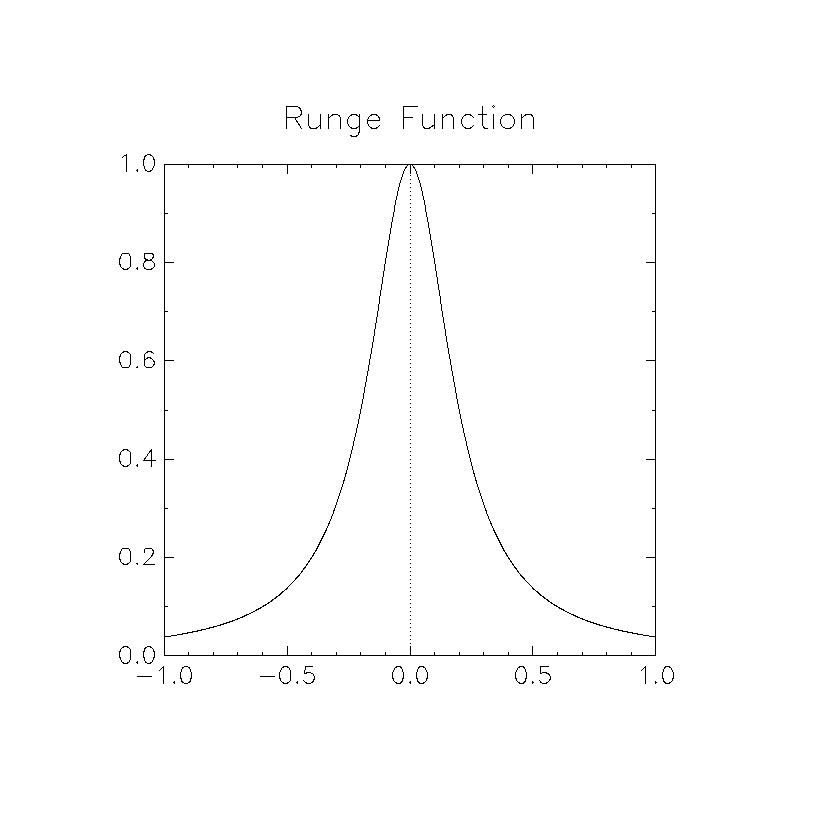
\includegraphics[width=9cm, trim={2cm, 4cm, 2cm, 3cm}, clip]{../images/runge}
        \caption{Runge function}
        \label{fig:runge}
    \end{figure}


\subsection{Polynomial through equidistant points}
\label{sec:firstpoly}
    We will start with Newton's divided differences interpolation to approximate the graph.
    A set of 17 equidistant points from -1 to 1 will be used do to the interpolation on, these will be generated as follows:
    \begin{lstlisting}
    int i = 0, size = 17;
    double xi, xa1[size], ya1[size];
    for (xi = -1; xi <= 1; xi = xi + ( 2 / (double) 16)) {
        xa1[i] = xi;
        ya1[i] = runge_f(xi);
        i++;
    }
    \end{lstlisting}
    To execute the interpolation, we need to initialize a couple of GSL structs.
    %\footnote{The initialization of these structs is analogue in the next sections, and will be omitted there.}
    \begin{lstlisting}
    gsl_interp_accel *acc = gsl_interp_accel_alloc();
    gsl_spline *interp_poly = gsl_spline_alloc(gsl_interp_polynomial, size);
    gsl_spline_init(interp_poly, xa1, ya1, size);
    \end{lstlisting}
    Here, the \href{https://www.gnu.org/software/gsl/manual/html_node/1D-Higher_002dlevel-Interface.html#g_t1D-Higher_002dlevel-Interface}
    {gsl\_spline} functions do not mean we are working with splines, despite what their name may suggest.
    They simply provide a higher level interface so that we can write less code later on. \\ The type of the interpolation
    we will work with is passed into the gsl\_spline\_alloc function. In this case, gsl\_spline\_init  will
    use gsl\_poly\_dd\_init to initialize the polynomial we will use. gsl\_poly\_dd\_init uses the Newton polynomial,
    which is what we need to calculate new interpolation points.

    Now, we can start plotting graphs. The gsl\_spline\_eval function is used to calculate new points. \\
    For each solution, we will plot 3 graphs: The result of the interpolation, and the absolute and relative difference
    with respect to the Runge function:
    \begin{lstlisting}
    double interpValue, realValue;
    for (xi = xa1[0]; xi < xa1[16]; xi += 0.001) {
        interpValue = gsl_spline_eval(interp_poly, xi, acc);
        realValue = runge_f(xi);
        file1 << xi << " " << interpValue << std::endl;
        file2 << xi << " " << interpValue - realValue << std::endl;
        file3 << xi << " " << (interpValue - realValue) / realValue << std::endl;
    }
    \end{lstlisting}
    The result of the interpolation and the difference with respect to the Runge function can be seen in figures~\ref{fig:poly1} and~\ref{fig:diff1}.
    %Graphs showing the relative differences can be found in the .zip file this report came in, they are omitted here as they do not bring

    \begin{figure}[H]
        \centering
        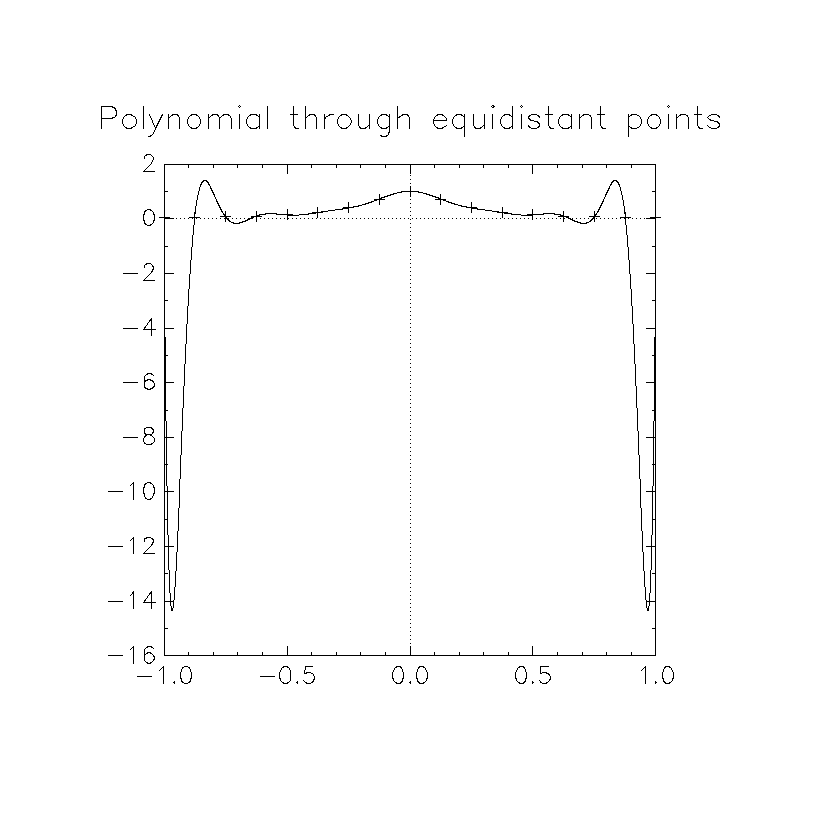
\includegraphics[width=9cm, trim={2cm, 4cm, 2cm, 3cm}, clip]{../images/poly1}
        \caption{Interpolation through equidistant points}
        \label{fig:poly1}
    \end{figure}
    At first glance, this approximation looks horrible. However, this is purely because of how the oscillations at the endpoints
    of the graph skew the graph. In the middle part of the graph, the approximation is pretty accurate.
    This is typical for interpolation polynomials of higher powers.
    \begin{figure}[H]
        \begin{minipage}[b]{0.49\textwidth}
            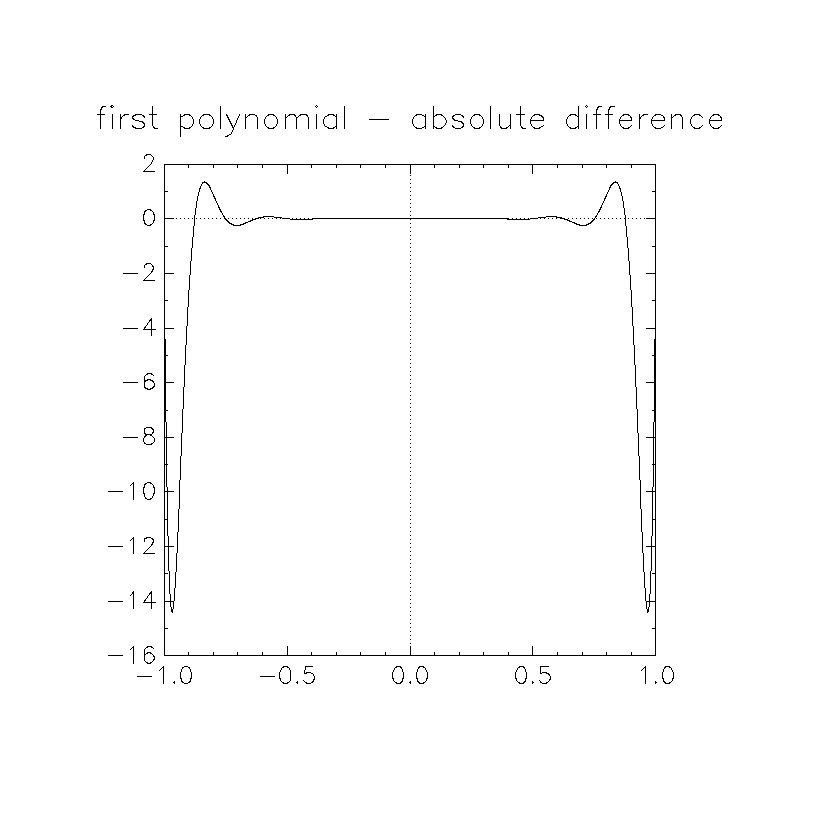
\includegraphics[width=6.5cm, trim={2cm, 4cm, 2cm, 3cm}, clip]{../images/diff1abs}
        \end{minipage}
        \hfill
        \begin{minipage}[b]{0.49\textwidth}
            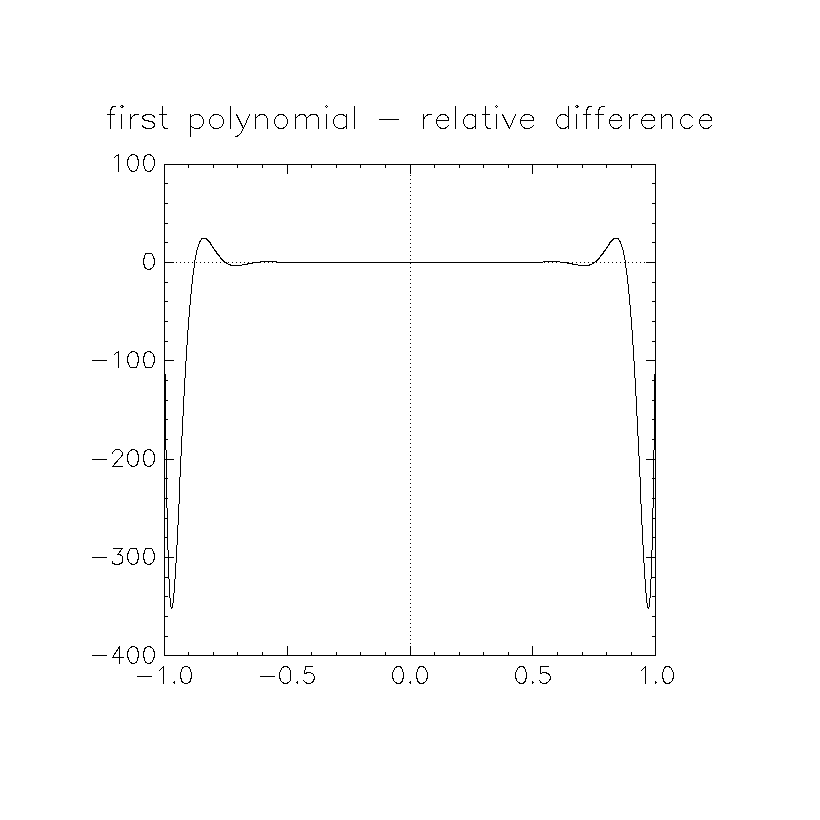
\includegraphics[width=6.5cm, trim={2cm, 4cm, 2cm, 3cm}, clip]{../images/diff1rel}
        \end{minipage}
        \caption{Differences for interpolation through equidistant points}
        \label{fig:diff1}
    \end{figure}
    In figure~\ref{fig:diff1}, it is clearly visible that the approximations are at their worst around the endpoints of the interpolation.

\subsection{Polynomial through non equidistant points}
    Now, we will apply the same method as in the previous section. The only difference lies in the set of points we use
    the interpolation on. This set is decided by \[x_i = \cos(\frac{(i + 0.5) \pi}{17}) \ \ where \ i \in \{0, 1, ..., 16\} \]
    \begin{lstlisting}
    for (i = 0; i <= 16; i++) {
        xa[i] = cos( ((double)i + 0.5) * (M_PI / 17) );
    }
    \end{lstlisting}
    The rest of the code is analogue to section~\ref{sec:firstpoly}. \\
    The result of using non equidistant points is instantly apparent in figures~\ref{fig:poly2} and~\ref{fig:diff2}.
    Compare them to figures~\ref{fig:poly1} and~\ref{fig:diff1} and you will see that using non equidistant points will
    dramatically improve the approximation, which is in line with what we have learned during the lectures on Scientific
    Programming. The oscillation is still present, but it is much less extreme now.
    \begin{figure}[H]
        \centering
        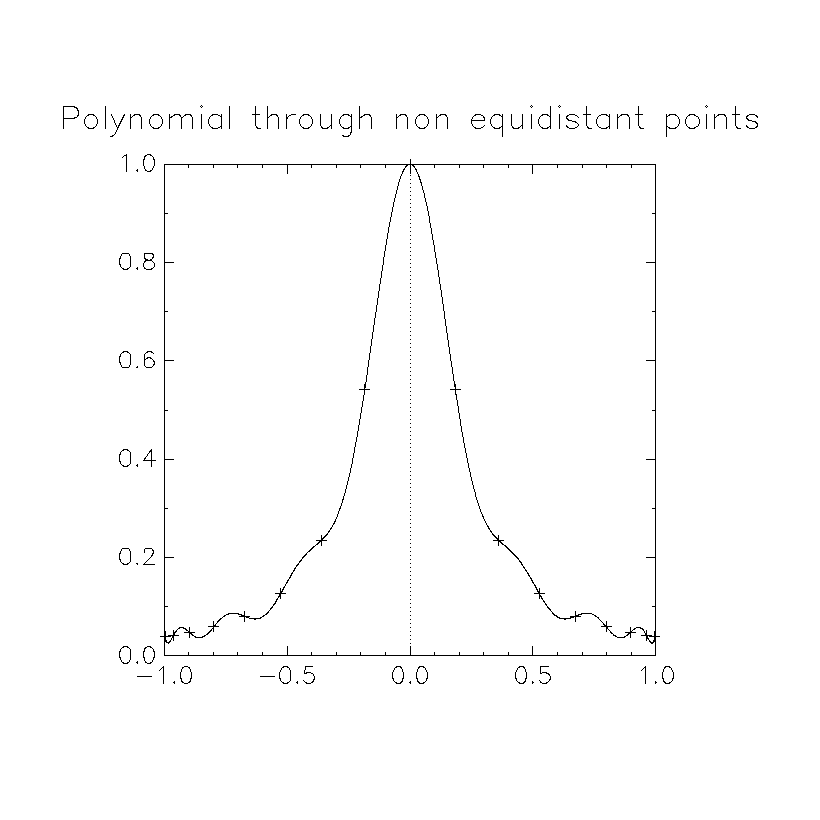
\includegraphics[width=9cm, trim={2cm, 4cm, 2cm, 3cm}, clip]{../images/poly2}
        \caption{Polynomial interpolation through non equidistant points}
        \label{fig:poly2}
    \end{figure}
    \begin{figure}[H]
        \begin{minipage}[b]{0.49\textwidth}
            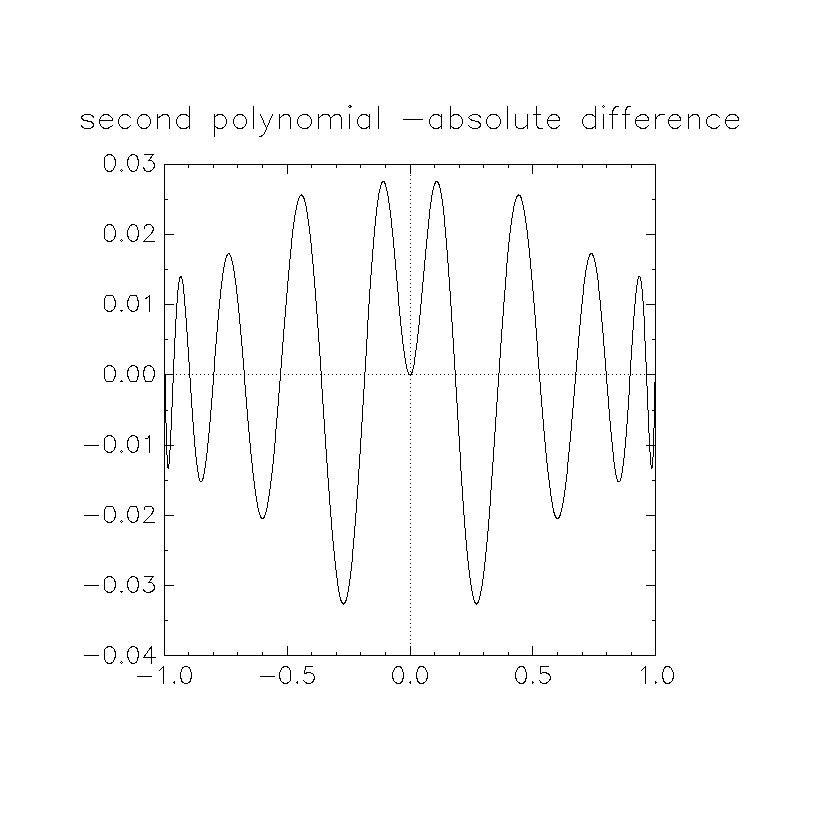
\includegraphics[width=6.5cm, trim={2cm, 4cm, 2cm, 3cm}, clip]{../images/diff2abs}
        \end{minipage}
        \hfill
        \begin{minipage}[b]{0.49\textwidth}
            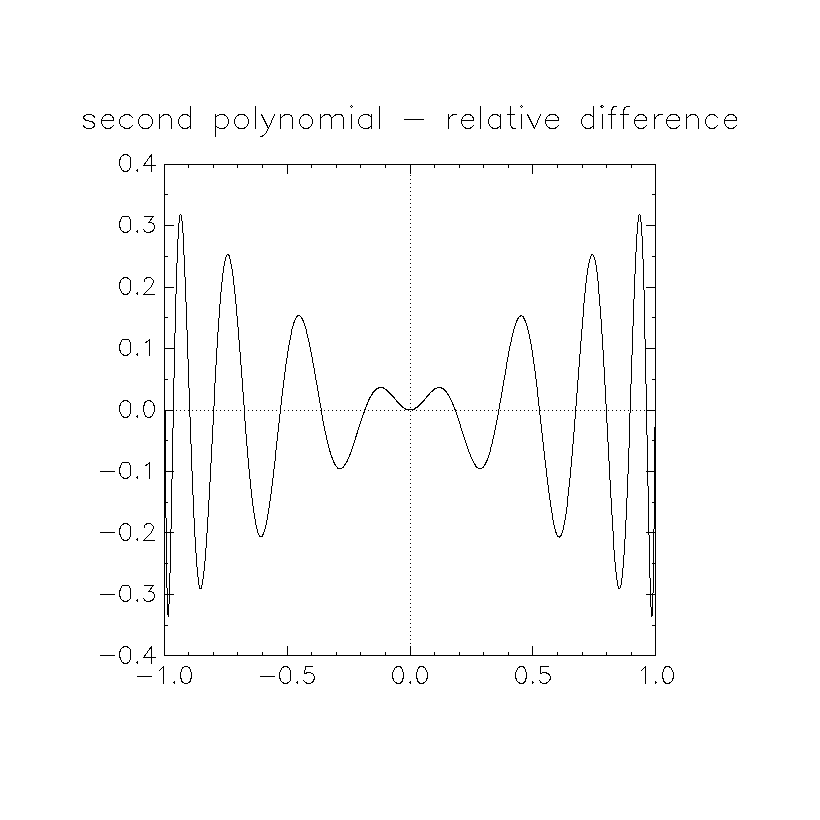
\includegraphics[width=6.5cm, trim={2cm, 4cm, 2cm, 3cm}, clip]{../images/diff2rel}
        \end{minipage}
        \caption{Differences for polynomial interpolation through non equidistant points}
        \label{fig:diff2}
    \end{figure}

\subsection{Natural cubic spline}
    GSL makes it simple to use various interpolation techniques. For natural cubic spline interpolation, the only difference
    we need in the code lies in the initialization of the interpolation struct. We can simply pass gsl\_interp\_cspline
    into gsl\_spline\_alloc instead of gsl\_interp\_polynomial. This will generate figures~\ref{fig:spline1}
    and~\ref{fig:diff3}.
    \begin{figure}[H]
        \centering
        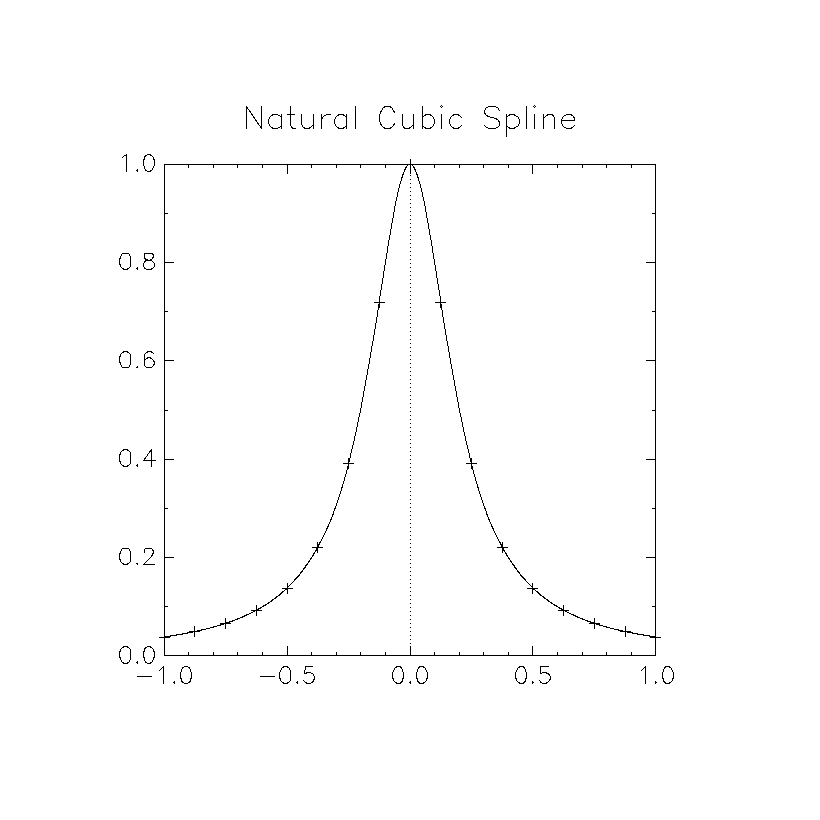
\includegraphics[width=9cm, trim={2cm, 4cm, 2cm, 3cm}, clip]{../images/spline1}
        \caption{Cubic spline interpolation through equidistant points}
        \label{fig:spline1}
    \end{figure}
    \begin{figure}[H]
        \begin{minipage}[b]{0.49\textwidth}
            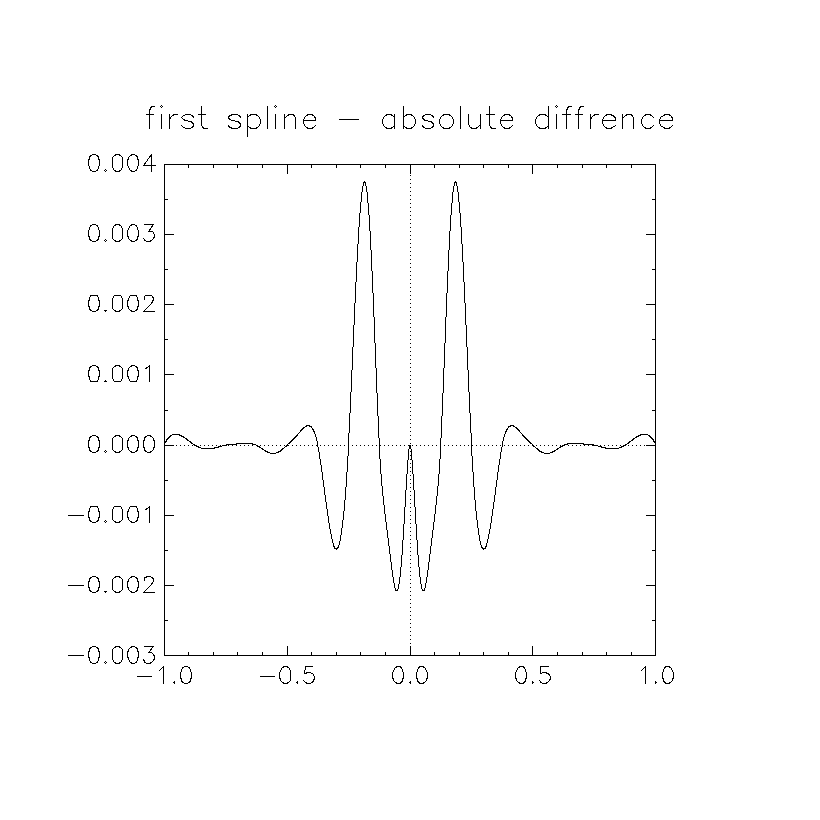
\includegraphics[width=6.5cm, trim={2cm, 4cm, 2cm, 3cm}, clip]{../images/diff3abs}
        \end{minipage}
        \hfill
        \begin{minipage}[b]{0.49\textwidth}
            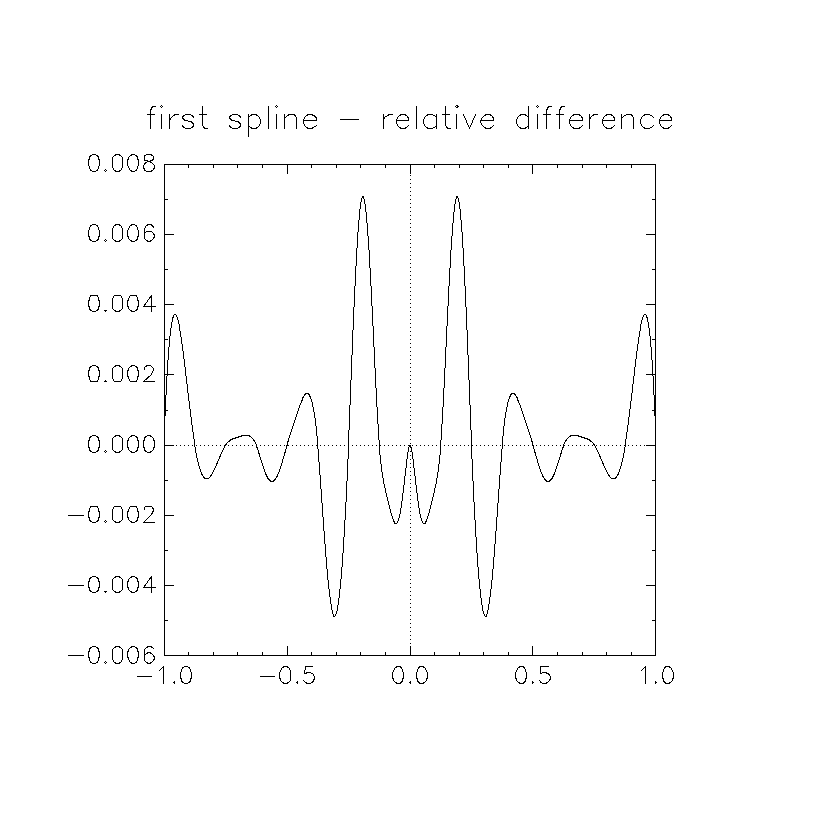
\includegraphics[width=6.5cm, trim={2cm, 4cm, 2cm, 3cm}, clip]{../images/diff3rel}
        \end{minipage}
        \caption{Differences for cubic spline interpolation}
        \label{fig:diff3}
    \end{figure}
    Spline interpolation can be used to avoid the extreme oscillations at the ends of intervals with polynomial interpolation.
    In figures~\ref{fig:spline1} and~\ref{fig:diff3}, We can see that the result of using a natural cubic spline looks almost identical to the runge function. The spline
    has produced a much better graph than both of the polynomials: its errors have a supremum of roughly 0.004,
    while for the polynomials this number is 14 and 0.03.

\subsection{Cubic spline with modified conditions}
    We now wish to execute a cubic spline interpolation with modified boundary conditions.
    We want to change the conditions to \[ S''(-1) = f''(-1) = \frac{925}{4394} \] and \[ S''(1) = f''(1) = \frac{925}{4394} \]
    However, there is no provided functionality to do this in GSL, so we will have to modify some of its code.
    In "cspline.c" in GSL's source code, we can see that in the cspline\_init function the boundary conditions are set to 0 for the cubic spline.
    \begin{lstlisting}
    106| state->c[0] = 0.0;
    107| state->c[max_index] = 0.0;
    \end{lstlisting}
    In our code we simply change these values after initializing the spline. To do this, we first need to copy the declaration
    for cspline\_state\_t into our code so we can access the conditions.
    \begin{lstlisting}
    gsl_spline *interp_spline = gsl_spline_alloc(gsl_interp_spline, size);
    gsl_spline_init(interp_spline, xa1, ya1, size);
    cspline_state_t *state = (cspline_state_t *) interp_cspline->interp->state;
    state->c[0] = (double) 925 / 4394;
    state->c[size - 1] = (double) 925 / 4394;
    \end{lstlisting}

    \bigskip
    The results are visible in figures~\ref{fig:spline2} and~\ref{fig:diff4}. The comparison of to the polynomial
    interpolation counts here as well, as not much has changed with respect to the natural cubic spline. Only the
    endpoints of the interval have changed, which is to be expected after changing the boundary conditions.
    The difference between the natural and this spline is only clear when looking at the graphs of the differences.
    In this case, we see that the difference with respect to the Runge function became worse when we modified the
    boundary conditions, which makes the natural cubic spline a better approximation.
    \begin{figure}[H]
        \centering
        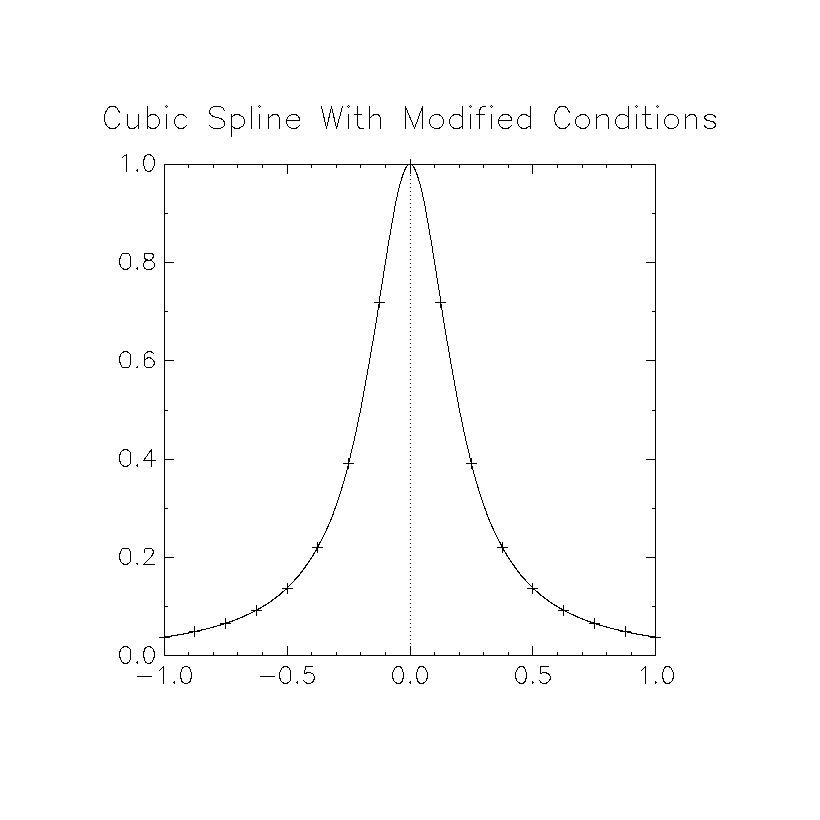
\includegraphics[width=9cm, trim={2cm, 4cm, 2cm, 3cm}, clip]{../images/spline2}
        \caption{Spline interpolation through equidistant points}
        \label{fig:spline2}
    \end{figure}
    \begin{figure}[H]
        \begin{minipage}[b]{0.49\textwidth}
            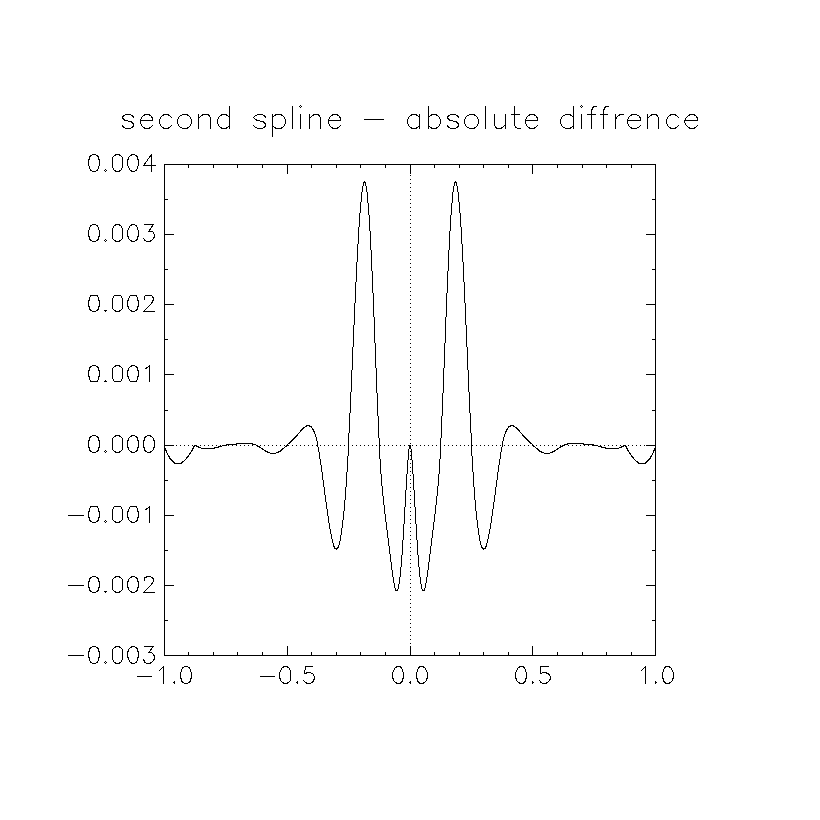
\includegraphics[width=6.5cm, trim={2cm, 4cm, 2cm, 3cm}, clip]{../images/diff4abs}
        \end{minipage}
        \hfill
        \begin{minipage}[b]{0.49\textwidth}
            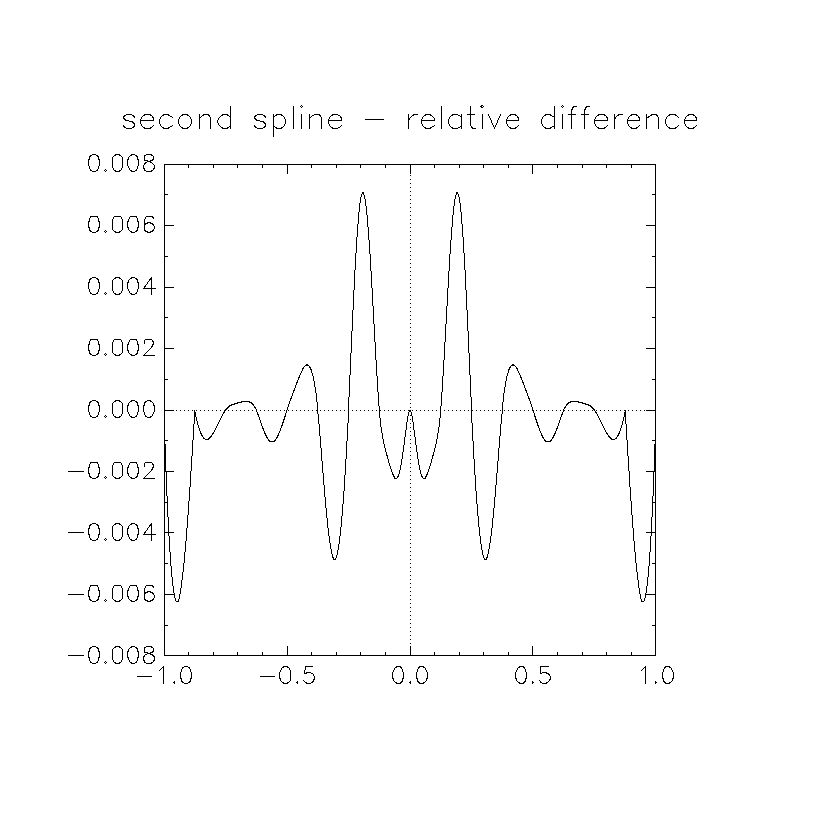
\includegraphics[width=6.5cm, trim={2cm, 4cm, 2cm, 3cm}, clip]{../images/diff4rel}
        \end{minipage}
        \caption{Differences for spline interpolation}
        \label{fig:diff4}
    \end{figure}


\section{Conclusion}
    After conducting the interpolations, we can conclude that using a cubic spline is the best way to
    approximate the Runge function, if we had to choose between polynomial and spline interpolation.
    This conforms to what we learned during the lecture on data fitting.

\onecolumn
\appendix
\appendixpage
\addappheadtotoc

\section{main.cpp}
    \lstinputlisting[basicstyle=\scriptsize]{../main.cpp}
    \newpage

\section{createImages.sh}
    \lstinputlisting[language=bash, basicstyle=\scriptsize]{../createImages.sh}

\end{document}